Resumen de diferentes partes: 

- Qué son los agentes, cómo interactúan con las herramientas y qué abstracciones ofrecen los frameworks que comentamos
- Ajuste de agentes -> LoRa?
- El protocolo MCP
- El estado del arte en arquitecturas de agentes LLM y sistemas RAG
- El estado del arte en agentes integrados a proyectos software

2. Agentes LLM (Fundamentos y funcionamiento básico)

¿Qué son los agentes LLM?
2.1. Modelos LLM
2.2. Interacción con herramientas
2.3. Abstracciones en frameworks

\section{Agentes LLM}

Los agentes IA son programas informáticos que utilizan modelos de Inteligencia Artificial para realizar diferentes tareas. Este tipo de agentes ha sido enfoque de investigación los últimos 75 años (todo). Debido a los últimos avances en el mundo del aprendizaje profundo, en los últimos años gran parte del esfuerzo se ha centrado en los agentes LLM.

\subsection{Modelos LLM}

Los modelos de lenguaje (LM), son modelos de inteligencia artificial que analizan y predicen texto. Tras varias decadas de avance, la investigación se ha focalizado en los Grandes Modelos de Lenguaje (LLM). Los LLM son modelos de lenguaje basados en redes neuronales, los cuales siguen la arquitectura Transformer [Attention is all you need]. 

A grandes rasgos, esta arquitectura utiliza el concepto de ``atención`` para enriquecer la comprensión que el modelo tiene sobre el texto. Para ello, el modelo primero transforma la respresentación de las palabras de entrada para que estas contengan información sobre el contexto de las demás palabras. Esto se consigue aplicando varias capas de atención, las cuales consisten en una serie de operaciones matriciales las cuales transfieren semántica entre las palabras. Tras obtener una representación enriquecida de las palabras, los modelos pueden realizar tareas como la generación, clasificación, traducción, etc.

Los agentes LLM utilizan en su mayoría modelos decodificadores autorregresivos, como GPT, Claude-Sonnet o Llama. Estos son un tipo de transformer focalizados en la generación de texto. Optimizados para la generación autorregresiva, la atención de cada token es sólo aplicada sobre los tokens anteriores. Esto permite que el modelo sólo calcule la atención que tokens anteriores aplican sobre el token actual, sin modificar la reresentación de los anteriores. 

La figura \ref{fig:atencion_gato} muestra un ejemplo simplificado del cómputo de atención para la frase ``El gato duerme``. Para generar la siguiente palabra, el modelo atenderá con diferentes magnitudes a la secuencia previa. En este caso, el modelo prestará más atención al hecho de que el gato esté durmiendo que al color del gato, por lo que la palabra  ``duerme`` tendrá más relevancia que la palabra ``negro`` a la hora de definir la semántica de la siguiente palabra. De esta forma, se calculará la probabilidad de la siguiente palabra teniendo en cuenta todo el vocabulario. De la misma forma, el modelo aplicó la influencia de las palabra ``El`` y ``gato`` para generar la palabra negro, pero no se le aplicará a la palabra ``gato`` la influencia de la palabra ``negro``.


\begin{figure}
    \centering
    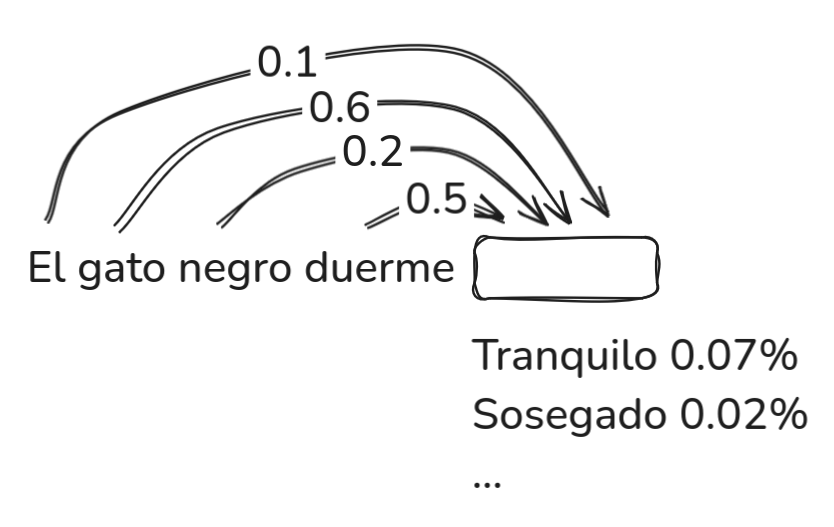
\includegraphics[width=0.65\linewidth]{figures/atencion_poc.png}
    \caption{Ejemplo simplificado de cómputo de atención para la frase \textquotedbl El gato duerme\textquotedbl}
    \label{fig:atencion_gato}
\end{figure}

\subsection{Interacción con herramientas}

\subsection{Abstraciones en frameworks}










